% \begin{figure}
%     \centering
%     \subfloat[DVS Circuit]{\label{fig:circuit}
%     \includegraphics[width=0.25\textwidth]{resources/images/intensity-estimation/DVSCircuit.png}}
%     \subfloat[3D Scene]{\label{fig:eyecatch:photo}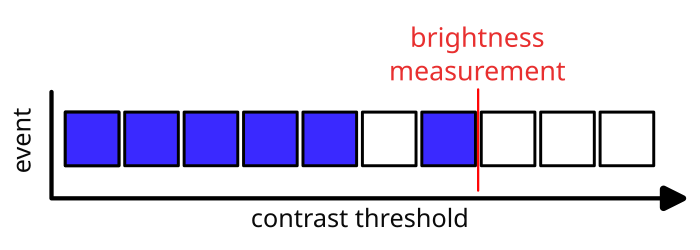
\includegraphics[width=0.2\textwidth]{resources/plots/intensity-estimation/scanning.png}
%     \caption[Schematic of the DVS Pixel Circuit]{Schematic of the DVS Pixel Circuit taken from \cite{DVSBiases2023}. It can be divided into a photoreceptor part (\textbf{A}), a source follower part (\textbf{B}) and a comparator part (\textbf{C} and \textbf{D})}
%     \label{fig:eventCircuit}
% \end{figure}

\begin{figure}
  \begin{subfigure}{0.5\textwidth}
    % \centering
    \includegraphics[height=2.4cm]{chapters/papers/ED/resources/images/intensity-estimation/DVSCircuit.png}
    \caption{}
    \label{fig:image1}
  \end{subfigure}
  \begin{subfigure}{0.5\textwidth}
    \centering
    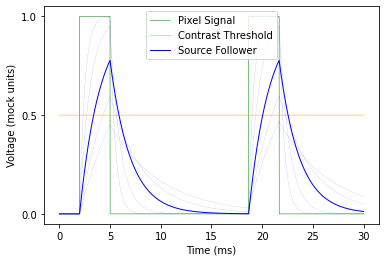
\includegraphics[width=0.7\linewidth]{chapters/papers/ED/resources/plots/intensity-estimation/source_follower.png}
    \caption{}
    \label{fig:image2}
  \end{subfigure}
  \caption{(a)Schematic of the DVS Pixel Circuit taken from \cite{DVSBiases2023}. It can be divided into a photoreceptor part (\textbf{A}), a source follower part (\textbf{B}) and a comparator part (\textbf{C} and \textbf{D})
  (b) }
  \label{fig:whole_figure}
\end{figure}